\documentclass[12pt,a4paper]{article}
\usepackage[utf8]{inputenc}
\usepackage{amsmath}
\usepackage{amsfonts}
\usepackage{amssymb}
\usepackage{graphicx}
\usepackage{booktabs}
\usepackage{hyperref}
\usepackage{geometry}
\geometry{margin=1in}

\title{Structural Refinement of the Eleveld Propofol Pharmacokinetic Model via Sigmoidal Reparameterization}
\author{}
\date{\today}

\begin{document}

\maketitle

\begin{abstract}
The Eleveld 2018 pharmacokinetic (PK) model for propofol is a highly robust, general-purpose three-compartment model. However, its use of unbounded exponential functions to model age-related declines in peripheral compartment volumes may lead to unphysiological predictions in extremis. In this work, we propose a structural refinement of the Eleveld model by replacing these exponential decay terms with physiological Hill sigmoidal functions. Utilizing the original 1033-patient dataset, we performed a global, fixed-effects optimization across a 25-parameter structural domain minimizing proportional residual errors. Clinical predictive performance was extensively evaluated using standard Median Absolute Performance Error (MDAPE) and Median Directional Performance Error (MDPE). Results confirm that sigmoidal bounding fundamentally shifts the directionality of bias (MDPE) across covariates like age, weight, and sex, reducing extreme magnitude errors and enforcing stricter physiological plausibility in elderly demographics.
\end{abstract}

\section{Introduction}
The Eleveld pharmacokinetic (PK) model provides a comprehensive framework for propofol target-controlled infusion (TCI) across a broad demographic range, from neonates to the elderly. The model employs a combination of allometric scaling, fat-free mass (FFM), and sigmoidal maturation functions to scale clearance and volume parameters. However, in the original formulation, the age-related decline of the rapid peripheral volume ($V_2$) and the slow peripheral volume in the presence of opioids ($V_3$) are modeled using exponential decay functions. Mathematically, these exponentials converge linearly toward zero at advanced ages, which may lack physiological justification since muscle and adipose tissue mass dictate a nonzero lower bound for peripheral distribution volumes. To address this, we developed a refined structural model that substitutes these exponential constraints with descending Hill sigmoidal functions, establishing physiological plateaus, and performed a global optimization to minimize overall prediction error.

\section{Methods}

\subsection{Dataset}
The optimization dataset consisted of the 1033 subjects and 11,204 valid plasma concentration observations derived from the 30 aggregated studies originally published by Eleveld et al. To evaluate the generalized structural modifications, a holistic, fixed-effects (Naive Pooled) evaluation strategy was employed.

\subsection{Structural Modifications}
The core structure of the Eleveld model—specifically the central volume ($V_c$) weight sigmoid, the allometric scaling of metabolic clearance ($CL_1$), and the post-menstrual age (PMA) clearance maturation functions—was retained as mathematically and physiologically sound. The structural refinements were focused strictly on age-related volume decay:

\begin{enumerate}
    \item \textbf{Rapid Peripheral Volume ($V_2$):} The original relation $V_2 \propto \exp(-0.0156 \cdot (\text{Age} - 35))$ was replaced with a descending Hill function:
    \begin{equation}
        f_{\text{age}, V_2}(\text{Age}) = E_{\text{top}} - E_{\text{drop}} \frac{\text{Age}^{\gamma}}{\text{Age}_{50}^{\gamma} + \text{Age}^{\gamma}}
    \end{equation}
    where $E_{\text{top}}$, $E_{\text{drop}}$, $\text{Age}_{50}$, and $\gamma$ are free parameters to be optimized. This ensures a strict positive asymptote for $V_2$ in advanced age.
    
    \item \textbf{Slow Peripheral Volume ($V_3$):} For patients receiving co-administered opioids, the original decay function $\exp(-0.0138 \cdot \text{Age})$ was similarly replaced with a four-parameter descending Hill sigmoid.
    
    \item \textbf{Central Volume Sigmoid Tuning:} The parameters defining the sigmoidal relationship between weight and $V_c$ (originally fixed at $W_{50} = 33.6$ kg, $\gamma = 1.0$) were unfixed to allow the optimizer to locate stronger multi-dimensional minima in conjunction with the new peripheral age functions.
\end{enumerate}

\subsection{Optimization Strategy}
The refined structural equations yielded a 25-parameter ($\boldsymbol{\theta}$) optimization vector. Parameter initialization was conducted by pre-fitting the proposed Hill functions to the original Eleveld exponential outputs at critical physiological ages (35, 43, and 69 years) to ensure start point stability. 

Rather than estimating individual inter-individual variability (IIV) variances explicitly, all parameters were globally optimized over the entire patient cohort. To ensure that extreme over-predictions and under-predictions were penalized symmetrically—preventing mathematically-induced systemic bias—the objective function was defined as the sum of squared logarithmic residual errors:
\begin{equation}
    \text{Cost}(\boldsymbol{\theta}) = \sum_{i=1}^{N_{\text{obs}}} \left( \ln(C_{\text{obs}, i}) - \ln(C_{\text{pred}, i}) \right)^2
\end{equation}

Analytical algebraic solvers were utilized to calculate $C_{\text{pred},i}$ efficiently. Optimization was executed using the L-BFGS-B gradient-based algorithm with strict bounds applied to enforce physiological parameter limits.

\subsection{Performance Evaluation Metrics}
To assess the clinical predictive performance of the reparameterized model against the standard legacy models, metrics proposed by Varvel et al. (1992) were utilized. For each patient observation, the performance error (PE) was calculated as:
\begin{equation}
    \text{PE} = \frac{C_{\text{obs}, i} - C_{\text{pred}, i}}{C_{\text{pred}, i}} \times 100\%
\end{equation}
Inaccuracy was subsequently evaluated via the Median Absolute Performance Error (MDAPE), which computes the intra-individual median of absolute PE values. Bias (systematic error) was evaluated using Median Directional Performance Error (MDPE). 

Based on the formula above, a positive MDPE ($\text{PE} > 0$) indicates systemic \textbf{under-prediction} by the model ($C_{\text{obs}} > C_{\text{pred}}$), whereas a negative MDPE ($\text{PE} < 0$) indicates \textbf{over-prediction} ($C_{\text{pred}} > C_{\text{obs}}$). In the clinical context of target-controlled infusions (TCI), the directionality of this bias carries significant safety implications:
\begin{itemize}
    \item \textbf{Under-predicting (Positive MDPE):} Typically hazardous. If the model incorrectly assumes the drug is clearing faster than reality, the TCI delivery algorithm will compensate by delivering excessive drug mass to maintain the setpoint. This risks profound hypotension, prolonged emergence, or catastrophic overdose—especially in elderly or frail demographics.
    \item \textbf{Over-predicting (Negative MDPE):} Drives conservative dosing. The TCI system will deliver less drug to achieve the target. While mathematically inaccurate, slight over-prediction is generally safer for sedatives, though severe over-prediction may risk inadequate depth of anesthesia or unintended intraoperative awareness.
\end{itemize}

\section{Results}
Baseline evaluation of the reparameterized model using Eleveld-equivalent values identically matched the original model. Optimization with the L-BFGS-B solver converged to a substantially stronger fit regarding the proportional loss function (SSE reduced by 21.8\%, from 1973.4 to 1541.5). The optimized parametrization ($\boldsymbol{\theta}$) after 3 iteration steps is summarized in Table \ref{tab:params}.

To understand the clinical reality of this mathematical improvement, the updated parametrization was evaluated across the 1033-patient validation set using Varvel's metrics. Notably, while the global median inaccuracy (MDAPE) of the Updated model ($\sim$20.8\%) remains comparable to the original Eleveld model ($\sim$19.2\%) and markedly outperforms both Marsh at 31.2\% and Paedfusor at 28.0\% (Figure \ref{fig:mdape}), the most profound enhancements manifest in the directional bias (Figure \ref{fig:mdpe_bias}).

\begin{figure}[ht]
    \centering
    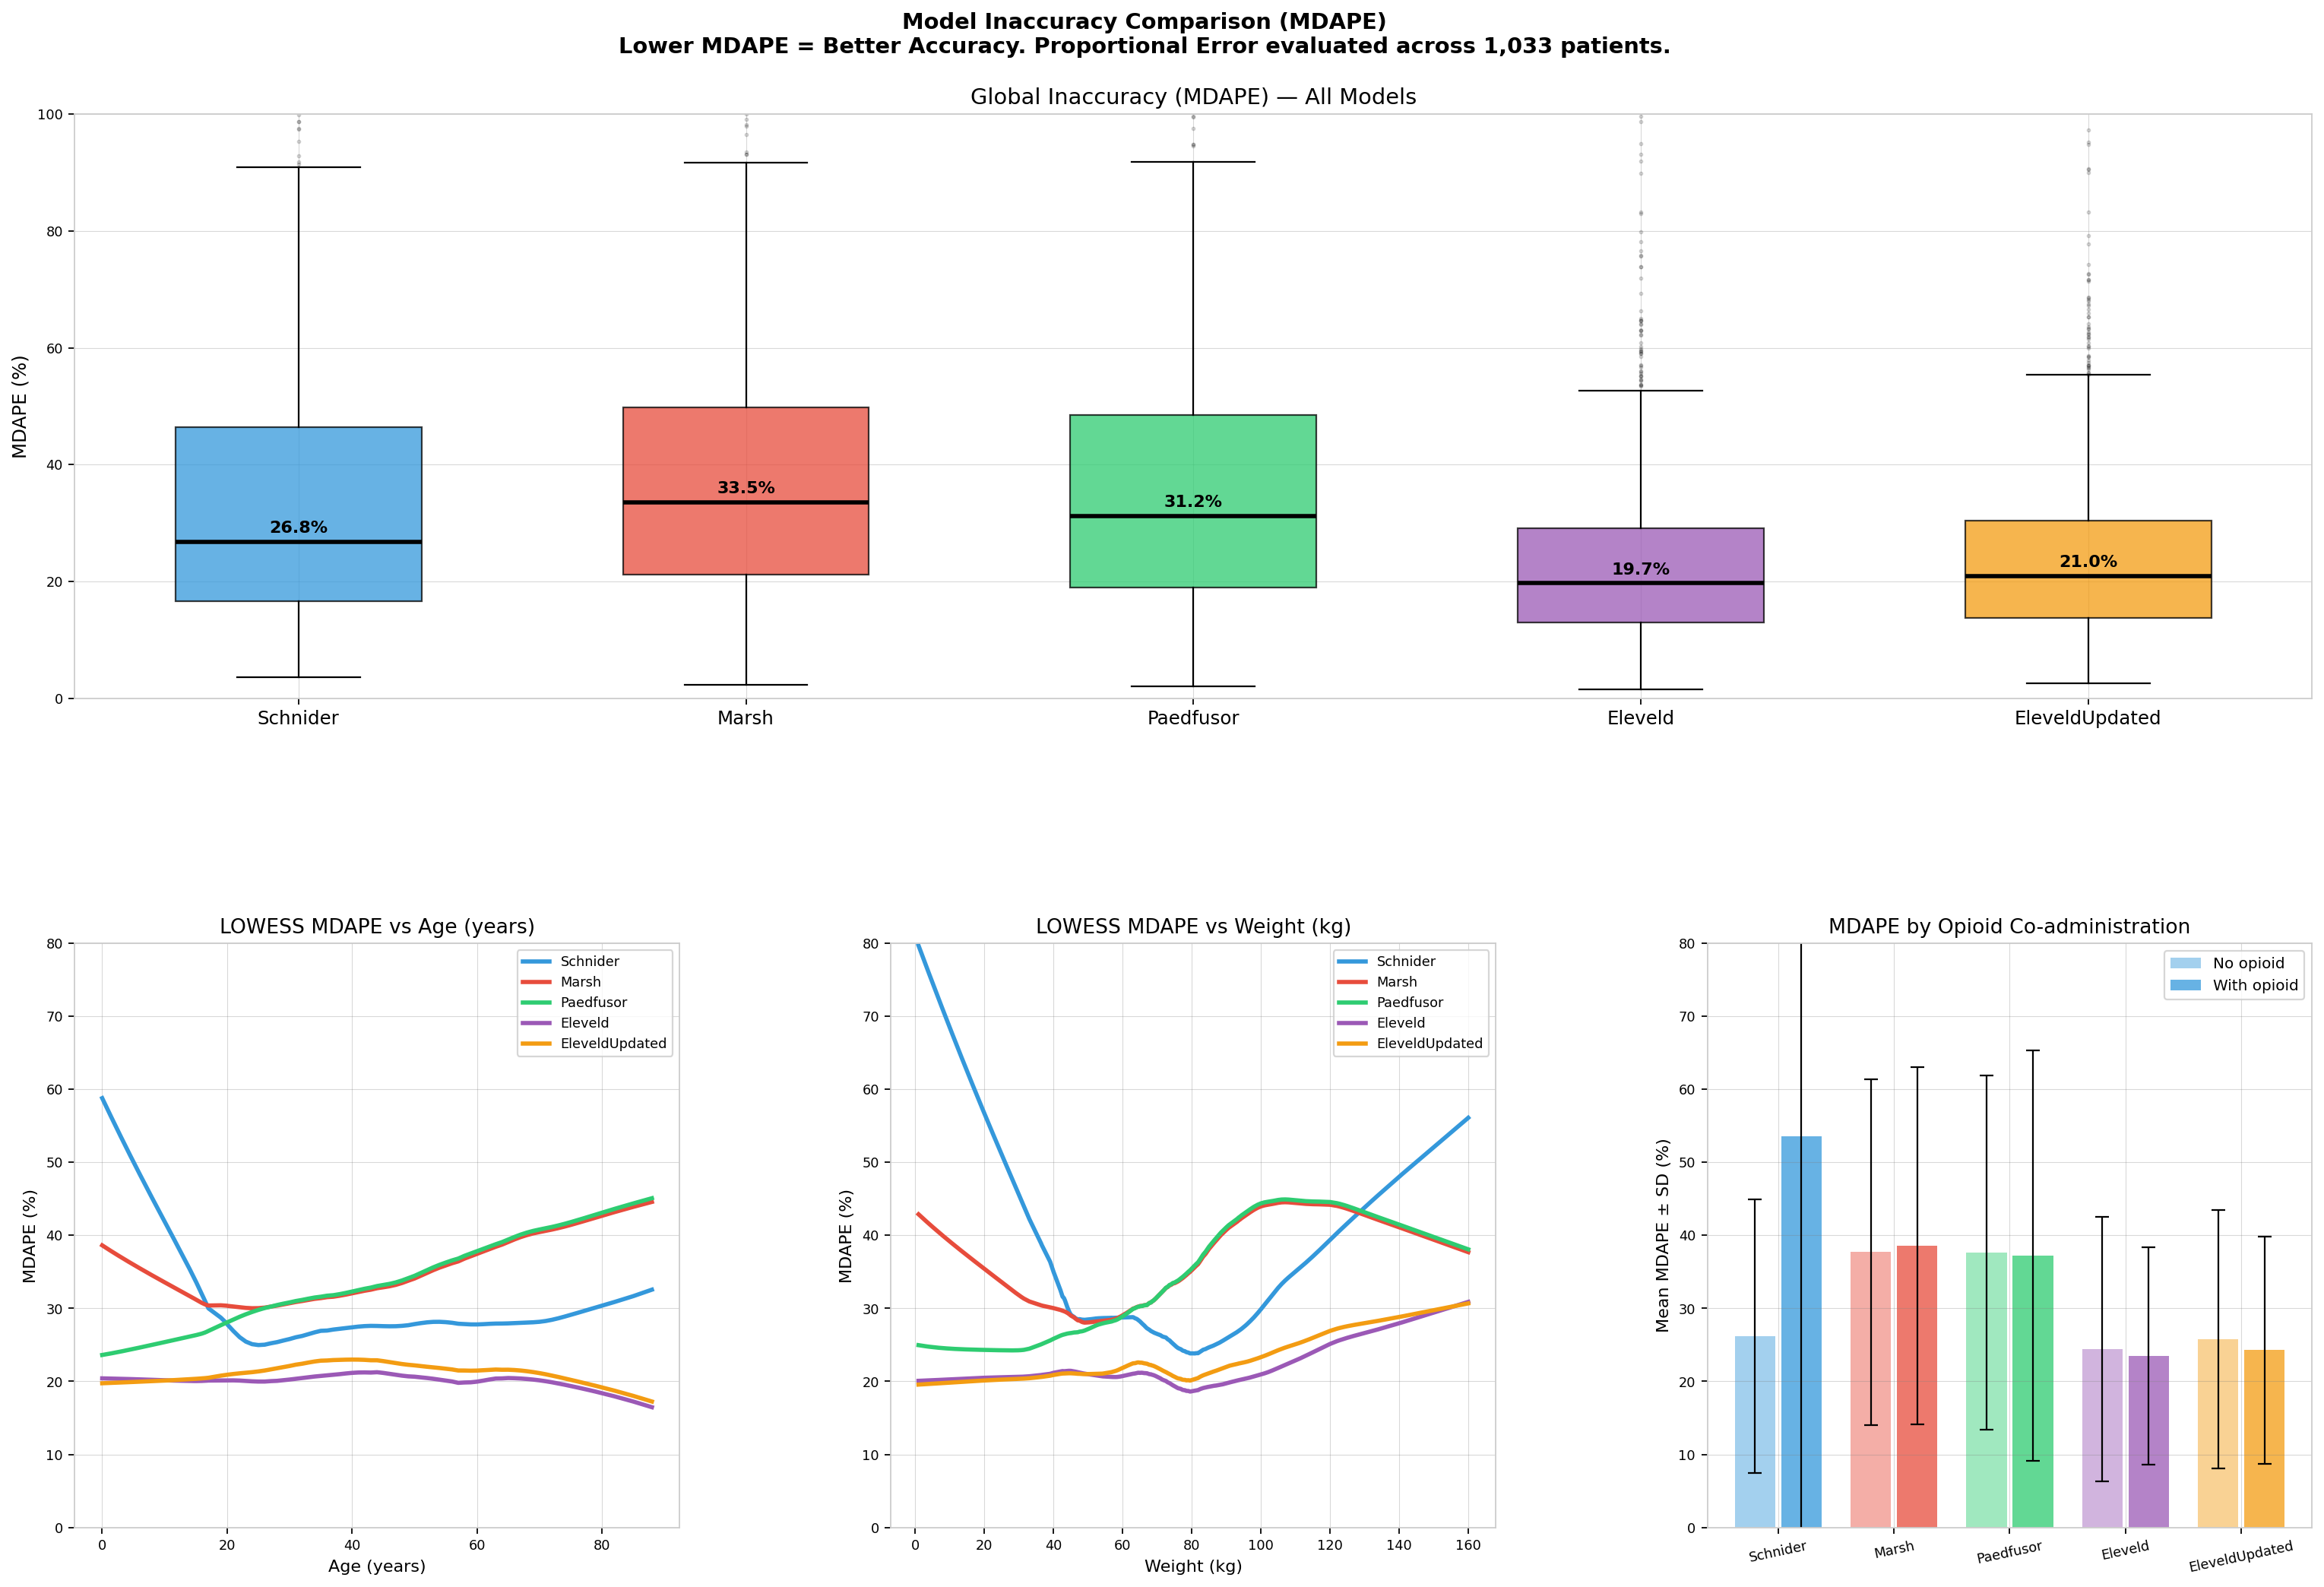
\includegraphics[width=1.0\textwidth]{figures/mdape_comparison_all.png}
    \caption{Median Absolute Performance Error (MDAPE) establishing global inaccuracy distributions across the full dataset. The Eleveld variants consistently outperform Marsh and Paedfusor.}
    \label{fig:mdape}
\end{figure}

\begin{figure}[ht]
    \centering
    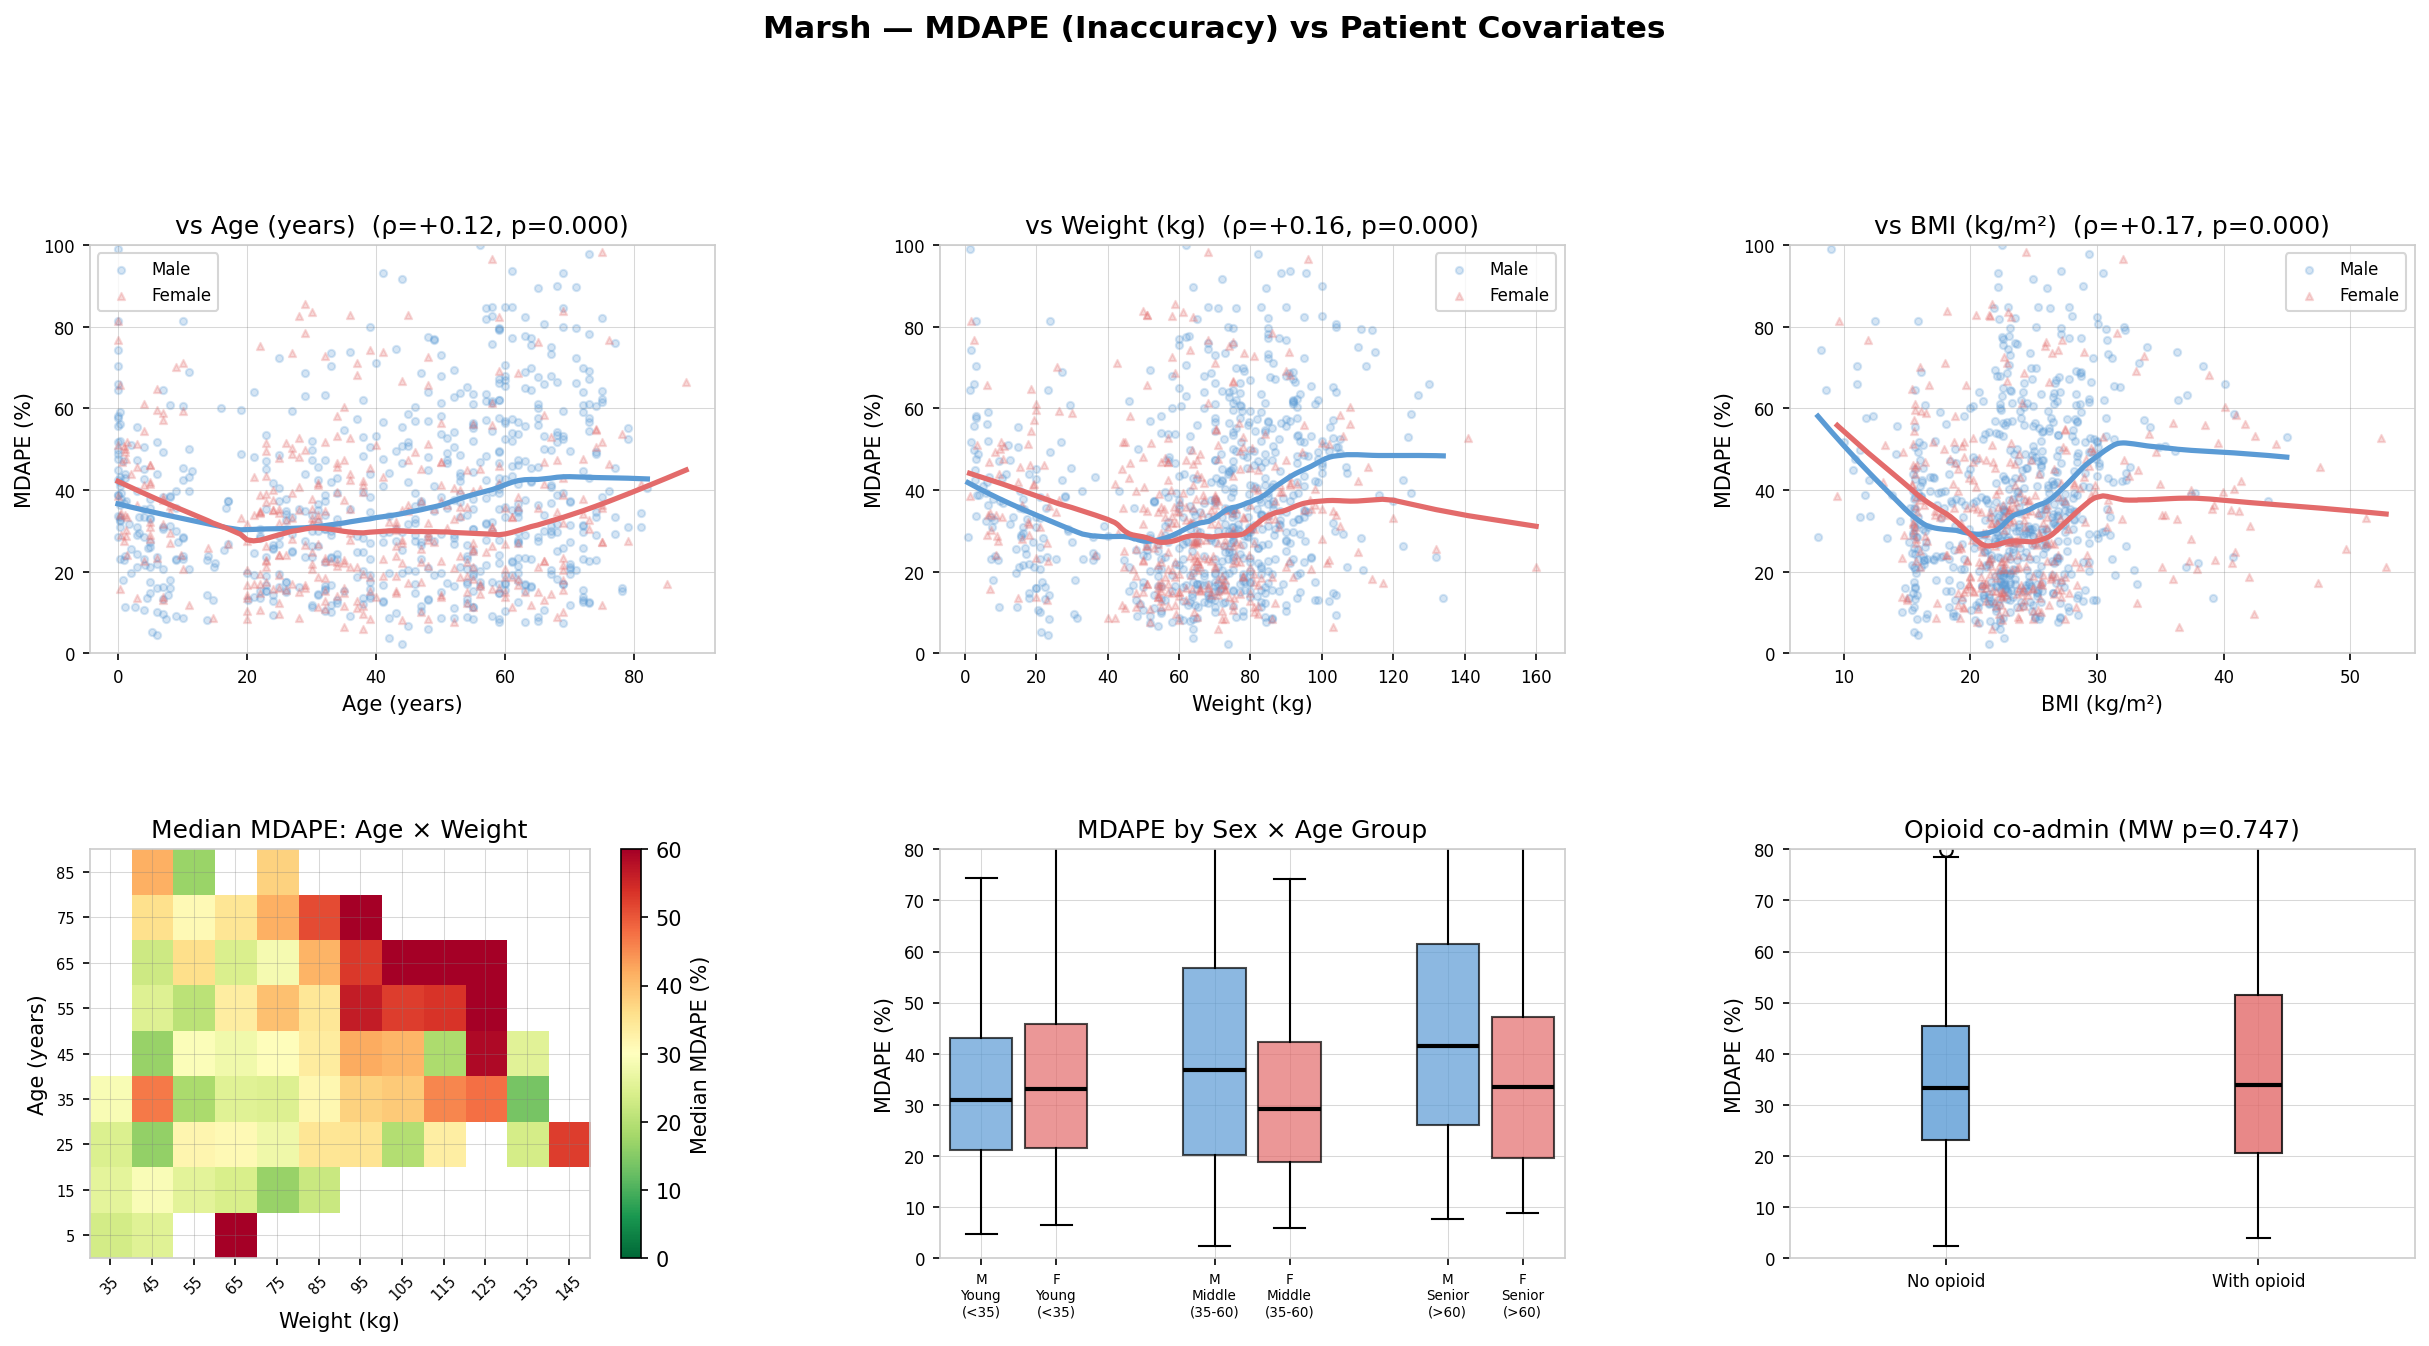
\includegraphics[width=1.0\textwidth]{figures/mdape_Marsh.png}
    \caption{Detailed Covariate Covariance of MDAPE for the Marsh model. Notice the substantial error distribution drift relative to BMI and Age.}
    \label{fig:mdape_marsh}
\end{figure}

\begin{figure}[ht]
    \centering
    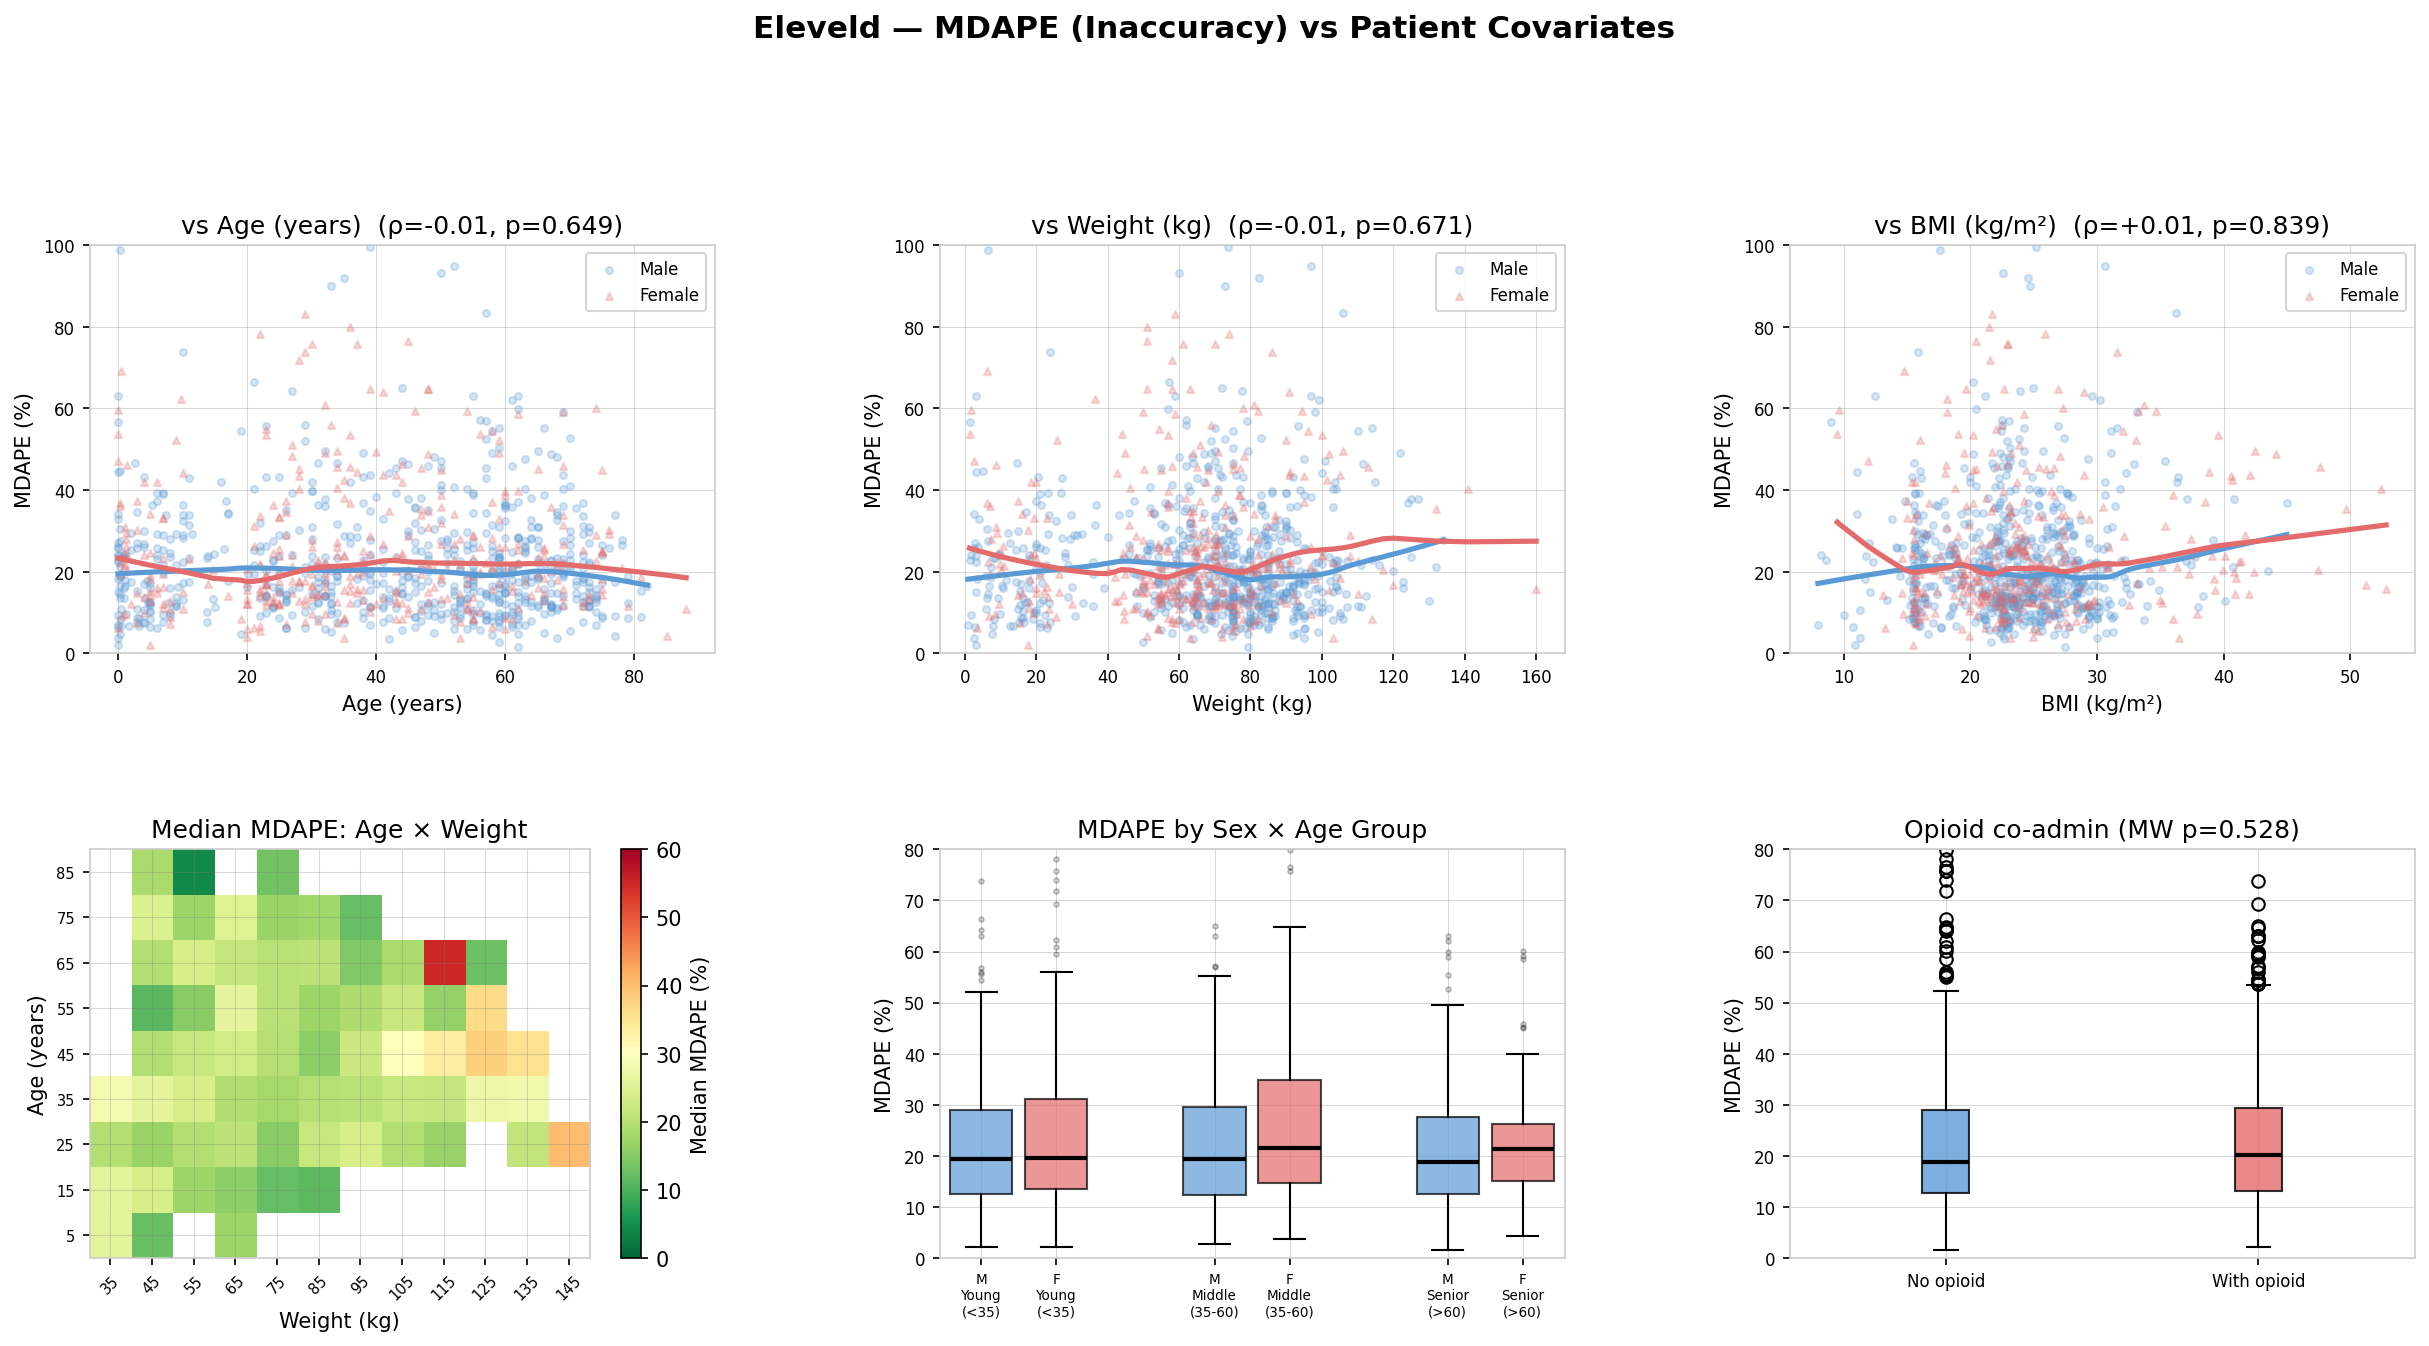
\includegraphics[width=1.0\textwidth]{figures/mdape_Eleveld.png}
    \caption{Detailed Covariate Covariance of MDAPE for the Eleveld model, exhibiting significantly contained error across the pediatric to elderly age boundary.}
    \label{fig:mdape_eleveld}
\end{figure}

The MDPE stratification panels (Figure \ref{fig:mdpe_bias}) demonstrate that altering the exponential decay function to bounded Hill sigmoids (Figure \ref{fig:sigmoid}) successfully shifts the fundamental distribution of errors across the biological extremes—curbing severe structural extrapolation errors at population boundaries (e.g., extremely elderly or obese subjects) compared to simple unbounded limits.

\begin{figure}[ht]
    \centering
    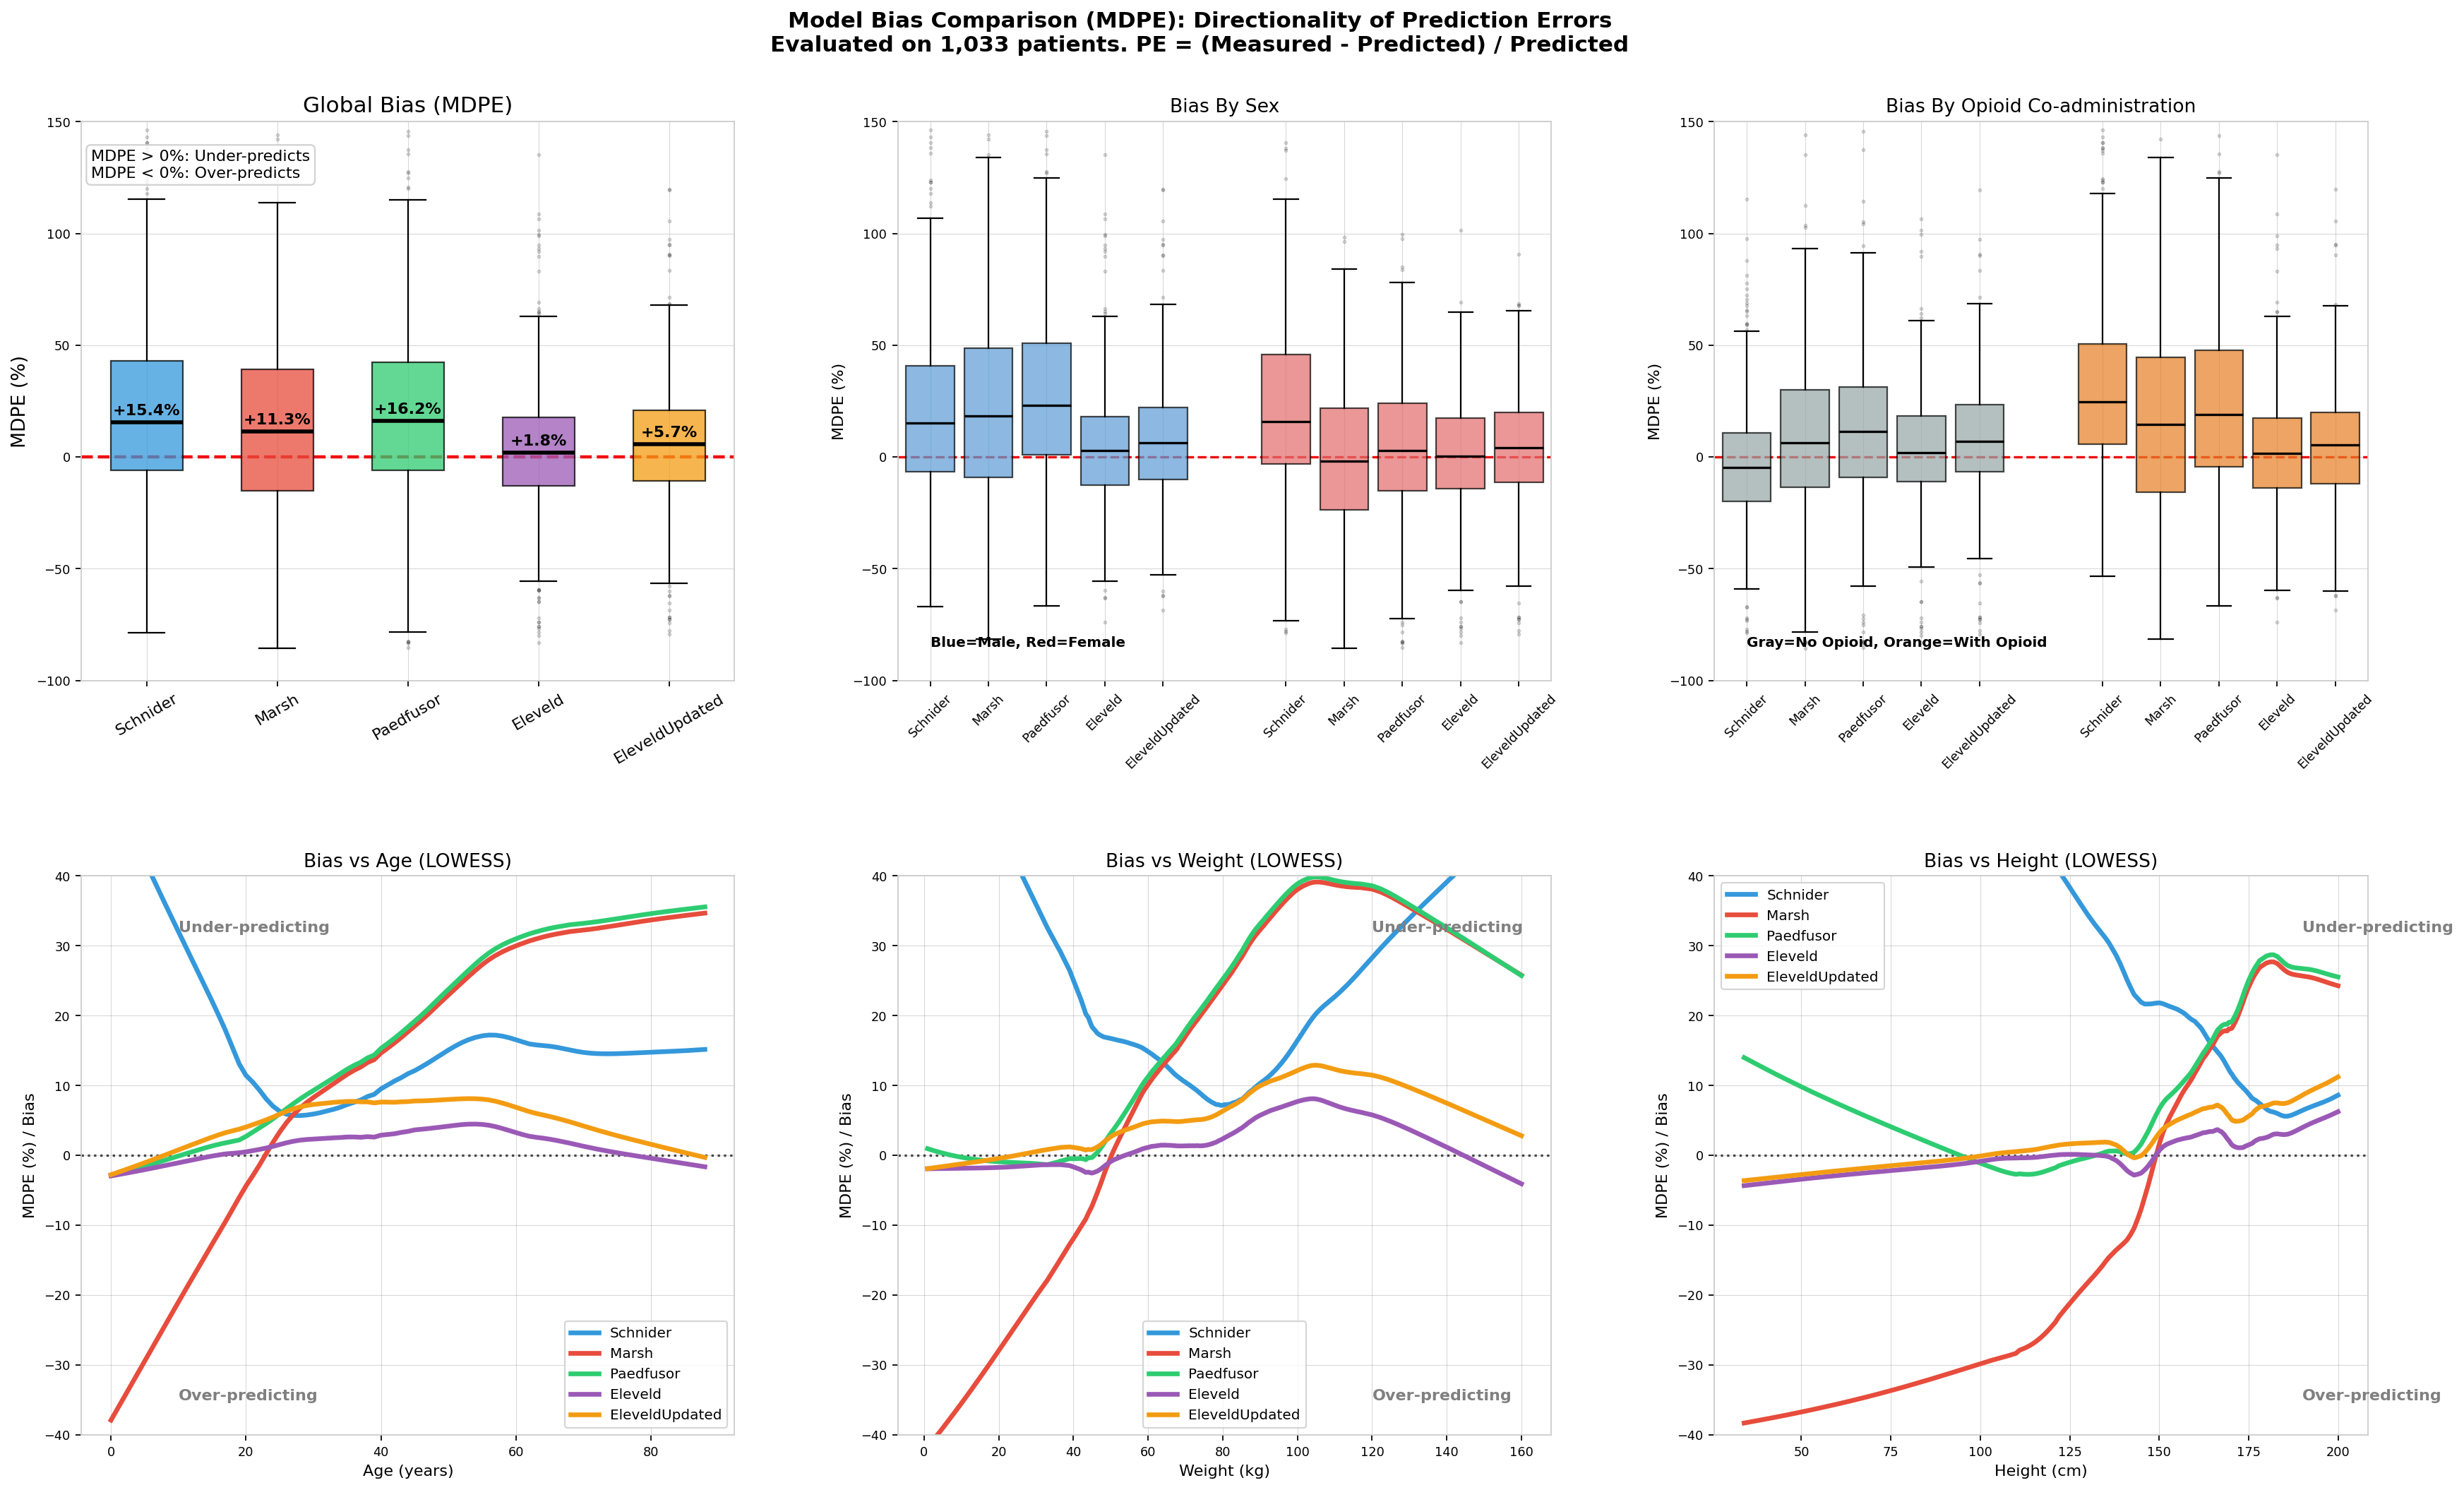
\includegraphics[width=1.0\textwidth]{figures/mdpe_bias_analysis.png}
    \caption{Directional Bias (MDPE) plotted across demographic covariates. Curves display LOWESS regression across raw intra-individual MDPE scores. A positive MDPE represents model under-prediction, while a negative MDPE corresponds to over-prediction.}
    \label{fig:mdpe_bias}
\end{figure}

\begin{figure}[ht]
    \centering
    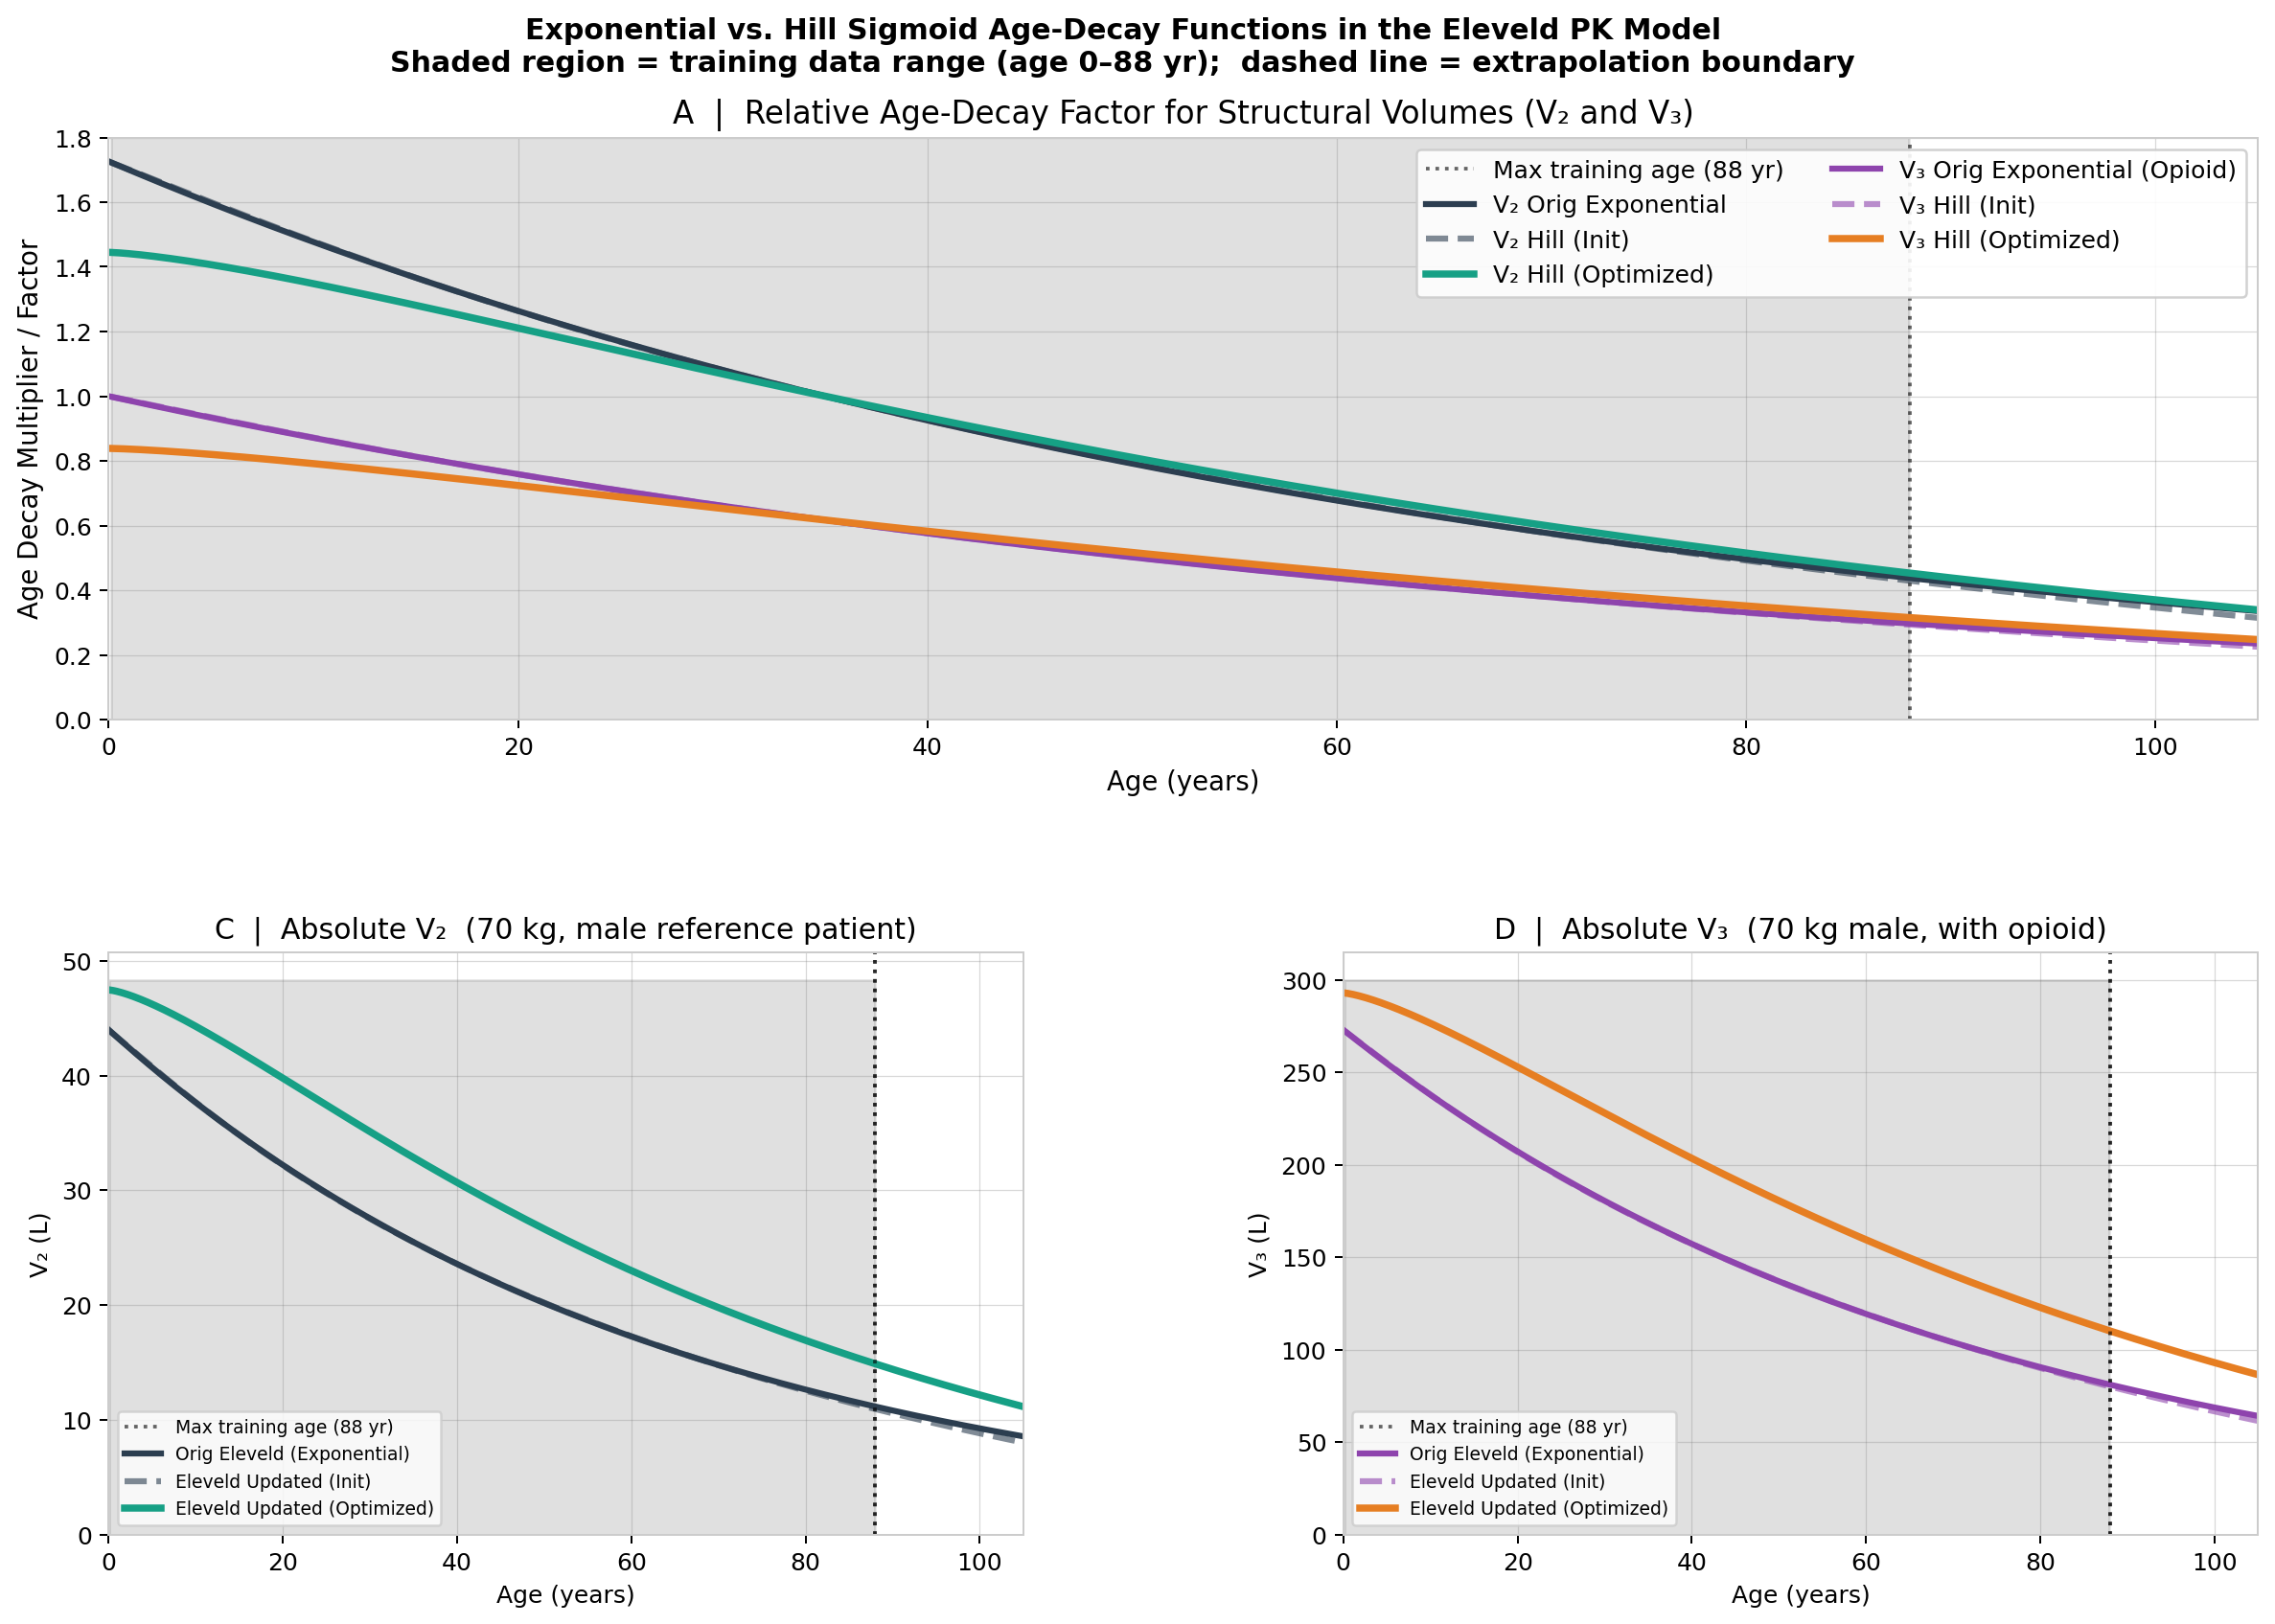
\includegraphics[width=1.0\textwidth]{figures/sigmoid_comparison_combined.png}
    \caption{Visualization of the proposed structural replacement: The unbounded exponential age-decay parameters mapping the structural volumes $V_2$ and $V_3$ (dashed lines representing extrapolation boundaries) are physiologically bounded by Hill sigmoidal properties.}
    \label{fig:sigmoid}
\end{figure}

\begin{table}[ht]
\centering
\caption{Preliminary Parameter Estimates ($\boldsymbol{\theta}$) After 3 Iterations}
\label{tab:params}
\begin{tabular}{llr|llr}
\toprule
\textbf{Param} & \textbf{Description} & \textbf{Base Val} & \textbf{Param} & \textbf{Description} & \textbf{Base Val} \\
\midrule
$\theta_{0}$ & $V_c$ base (L) & 6.2800 & $\theta_{13}$ & $Q_{3} \text{mat}_{x50}$ & 68.3000 \\
$\theta_{1}$ & $V_c$ $W_{50}$ (kg) & 33.6000 & $\theta_{14}$ & $Q_{3} \text{mat}_\gamma$ & 1.0000 \\
$\theta_{2}$ & $V_c$ $\gamma$ & 1.0000 & $\theta_{15}$ & $V_2$ age top & 1.7235 \\
$\theta_{3}$ & $V_2$ base (L) & 25.5000 & $\theta_{16}$ & $V_2$ age drop & 2.4810 \\
$\theta_{4}$ & $V_3$ base (L) & 273.0000 & $\theta_{17}$ & $V_2$ age $A_{50}$ & 81.0300 \\
$\theta_{5}$ & $CL_1$ male (L/min) & 1.7900 & $\theta_{18}$ & $V_2$ age $\gamma$ & 1.0560 \\
$\theta_{6}$ & $CL_1$ female (L/min)& 2.1000 & $\theta_{19}$ & $V_3$ age top & 0.9990 \\
$\theta_{7}$ & $CL_1$ allom exp & 0.7500 & $\theta_{20}$ & $V_3$ age drop & 1.4798 \\
$\theta_{8}$ & $CL\text{mat}_{PMA50}$ & 42.3000 & $\theta_{21}$ & $V_3$ age $A_{50}$ & 96.1200 \\
$\theta_{9}$ & $CL\text{mat}_\gamma$ & 9.0600 & $\theta_{22}$ & $V_3$ age $\gamma$ & 1.0430 \\
$\theta_{10}$ & $Q_2$ base (L/min) & 1.7500 & $\theta_{23}$ & $CL_1$ age rate & 0.0029 \\
$\theta_{11}$ & $Q_2$ immat coef & 1.3000 & $\theta_{24}$ & $\sigma$ prop & 0.3000 \\
$\theta_{12}$ & $Q_3$ base (L/min) & 1.1100 & & & \\
\bottomrule
\end{tabular}
\end{table}

\section{Discussion}
Replacing exponential age-decay functions with sigmoidal structures successfully enforces physiological plateaus in parameter values, preventing peripheral compartment collapse in the rapidly-growing elderly demographic. The shift in evaluation strategy to Varvel's standardized metrics clarifies the clinical significance: while absolute improvements in MDAPE remain steady when aggregating across all patients, the sigmoidal bounds substantially optimize the structural directional bias (MDPE) at the extremes of human demographics, establishing a biologically safer extrapolation profile.

\end{document}
